\documentclass[a4paper,10pt]{report}
\usepackage[utf8]{inputenc}
\usepackage{graphicx}

% Title Page
\title{}
\author{}


\begin{document}

\section*{\textit{Layered Label Propagation Distribúido}(Esboço)}

Cada vértice terá:
\begin{itemize}
  \item A sua \textit{label}
\end{itemize}

\begin{figure}[h]
\center
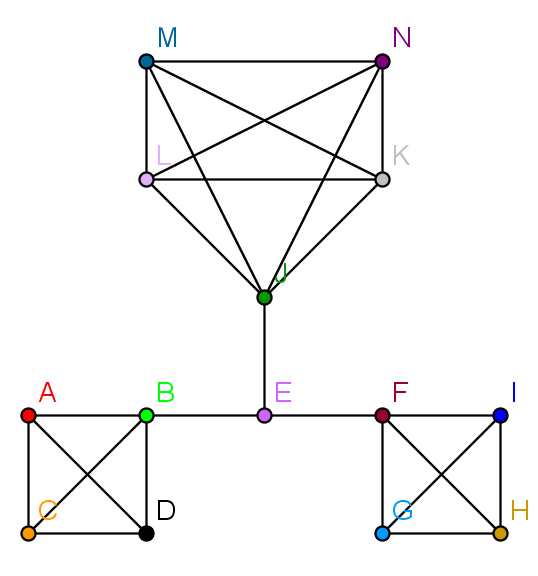
\includegraphics{graph_step0}
\caption{Grafo de exemplo.\label{fig:distributedexample1}}
\end{figure}

{\bf Exemplo para o grafo da figura \ref{fig:distributedexample1}}
\\[0.25cm]
{\bf Fase de preparação:}\\
Todos os vértices ficam com uma $label$ única. 
\\[0.25cm]
{\bf \textit{Superstep} 0  (1º Passo do algoritmo):}
Não receberam mensagens, logo não precisam de fazer \textit{update} ao sei 
$v_i$.
Os vértices enviam para os seus adjacentes 
informação sobre a sua \textit{label} e com $v_i=1$.
\\[0.25cm]
{\bf \textit{Superstep} 1 (2º Passo do algoritmo):}
Os vértices recebem as mensagens enviadas pelos seus adjacentes e calculam a 
$label_i$ que é maximizada na sua vizinhança. Iteração$ = (1/3) mod 3\approx0$, 
logo os vértices não iram se juntar a comunidades cuja $label$ seja menor à que 
têm.
\\[0.25cm]
Vértice A:
  \begin{tabular}{| l | l | l | l |}
  \hline
  $label_i$ & $k_i$ & $v_i$ & $k_i - \gamma(v_i - k_i)$\\ \hline
  A & 1 & 0 & 1 \\ \hline
  B & 1 & 1 & 1  \\ \hline
  C & 1 & 1 & 1  \\ \hline
  D & 1 & 1 & 1  \\ \hline
  \end{tabular}
  A fica com a \textit{label} B.
\\[0.25cm]
Neste passo apenas o vértice A muda, porque apenas A muda para um vértice cuja 
$label$ é maior que a sua. Este passo previne o acontecimento de ciclos.
\\[0.25cm]
{\bf \textit{Superstep} 2 (3º Passo do algoritmo):} Os vértices representantes 
de cada comunidade calculam o $v_i$ atualizado para a sua $label_i$ e devolvem 
para os seus membros.
\\[0.25cm]
Vértice B:
  \begin{tabular}{| l | l | l | l |}
  \hline
  $From Vid$ & $label_i$\\ \hline
  A & B \\ \hline
  B & B \\ \hline
  \end{tabular}  
\\[0.25cm]
  Envia $v_B = 2$ para os vértices A e B.
  
  Todos os outros vértices recebem uma mensagem de si próprios e enviam 
$v_i=1$ de volta para si.
\\[0.25cm]
{\bf \textit{Superstep} 3 (1º Passo do algoritmo):}
Receberam mensagens, logo iram meter o seu $v_i$ igual ao que receberam.
Os vértices enviam para os seus adjacentes informação sobre a sua 
\textit{label} e com $v_i=1$.
\\[0.25cm] 
{\bf \textit{Superstep} 4 (2º Passo do algoritmo):}
Iteração$ = (4/3) mod 3\approx1$, 
logo os vértices podem-se juntar a comunidades cuja $label$ seja menor à que 
têm.
\\[0.25cm]
Vértice A:
  \begin{tabular}{| l | l | l | l |}
  \hline
  $label_i$ & $k_i$ & $v_i$ & $k_i - \gamma(v_i - k_i)$\\ \hline
  B & 2 & 2 & 2 \\ \hline
  C & 1 & 1 & 1 \\ \hline
  D & 1 & 1 & 1 \\ \hline
  \end{tabular}
  A fica com a \textit{label} B.
\\[0.25cm]
Vértice B:
  \begin{tabular}{| l | l | l | l | l |}
  \hline
  $label_i$ & $k_i$ & $v_i$ & $k_i - \gamma(v_i - k_i)$\\ \hline
  B & 2 & 2 & 2 \\ \hline
  C & 1 & 1 & 1  \\ \hline
  D & 1 & 1 & 1  \\ \hline
  \end{tabular}
  B fica com a \textit{label} B.
\\[0.25cm]
Vértice C:
  \begin{tabular}{| l | l | l | l |}
  \hline
  $label_i$ & $k_i$ & $v_i$ & $k_i - \gamma(v_i - k_i)$\\ \hline
  B & 2 & 2 & 2 \\ \hline
  C & 0 & 1 & -1 \\ \hline
  D & 1 & 1 & 1 \\ \hline
  \end{tabular}
  C fica com a \textit{label} B.
\\[0.25cm]
Vértice D:
  \begin{tabular}{| l | l | l | l |}
  \hline
  $label_i$ & $k_i$ & $v_i$ & $k_i - \gamma(v_i - k_i)$\\ \hline
  B & 2 & 2 & 2  \\ \hline
  C & 1 & 1 & 1  \\ \hline
  D & 0 & 1 & -1 \\ \hline
  \end{tabular}  
  D fica com a \textit{label} B.
\\[0.25cm]
Vértice E:
  \begin{tabular}{| l | l | l | l |}
  \hline
  $label_i$ & $k_i$ & $v_i$ & $k_i - \gamma(v_i - k_i)$\\ \hline
  E & 0 & 1 & -1 \\ \hline
  B & 1 & 2 & 0  \\ \hline
  F & 1 & 1 & 1  \\ \hline
  J & 1 & 1 & 1  \\ \hline
  \end{tabular}  
  E fica com a \textit{label} F.
\\[0.25cm]
Vértice F:
  \begin{tabular}{| l | l | l | l |}
  \hline
  $label_i$ & $k_i$ & $v_i$ & $k_i - \gamma(v_i - k_i)$\\ \hline
  F & 0 & 1 & -1 \\ \hline
  E & 1 & 1 & 1  \\ \hline
  I & 1 & 1 & 1  \\ \hline
  G & 1 & 1 & 1  \\ \hline
  H & 1 & 1 & 1  \\ \hline
  \end{tabular}  
  F fica com a \textit{label} E.
\\[0.25cm]
Vértice G:
  \begin{tabular}{| l | l | l | l |}
  \hline
  $label_i$ & $k_i$ & $v_i$ & $k_i - \gamma(v_i - k_i)$\\ \hline
  G & 0 & 1 & -1 \\ \hline
  I & 1 & 1 & 1  \\ \hline
  F & 1 & 1 & 1  \\ \hline
  H & 1 & 1 & 1  \\ \hline
  \end{tabular}  
  G fica com a \textit{label} F.
\\[0.25cm]
Vértice H:
  \begin{tabular}{| l | l | l | l |}
  \hline
  $label_i$ & $k_i$ & $v_i$ & $k_i - \gamma(v_i - k_i)$\\ \hline
  H & 1 & 1 & -1  \\ \hline
  I & 0 & 1 & 1 \\ \hline
  F & 1 & 1 & 1  \\ \hline
  G & 1 & 1 & 1  \\ \hline
  \end{tabular}  
  H fica com a \textit{label} F.
\\[0.25cm]
Vértice I:
  \begin{tabular}{| l | l | l | l |}
  \hline
  $label_i$ & $k_i$ & $v_i$ & $k_i - \gamma(v_i - k_i)$\\ \hline
  I & 0 & 1 & -1 \\ \hline
  F & 1 & 1 & 1  \\ \hline
  G & 1 & 1 & 1  \\ \hline
  H & 1 & 1 & 1  \\ \hline
  \end{tabular}  
  I fica com a \textit{label} F.
\\[0.25cm]
Vértice J:
  \begin{tabular}{| l | l | l | l |}
  \hline
  $label_i$ & $k_i$ & $v_i$ & $k_i - \gamma(v_i - k_i)$\\ \hline
  J & 0 & 1 & -1 \\ \hline
  E & 1 & 1 & 1  \\ \hline
  K & 1 & 1 & 1  \\ \hline
  L & 1 & 1 & 1  \\ \hline
  M & 1 & 1 & 1  \\ \hline
  N & 1 & 1 & 1  \\ \hline
  \end{tabular}  
  J fica com a \textit{label} E.
\\[0.25cm]
Vértice K:
  \begin{tabular}{| l | l | l | l |}
  \hline
  $label_i$ & $k_i$ & $v_i$ & $k_i - \gamma(v_i - k_i)$\\ \hline
  K & 0 & 1 & -1 \\ \hline
  J & 1 & 1 & 1  \\ \hline
  L & 1 & 1 & 1  \\ \hline
  M & 1 & 1 & 1  \\ \hline
  N & 1 & 1 & 1  \\ \hline
  \end{tabular}  
  K fica com a \textit{label} J.
\\[0.25cm]
Vértice L:
  \begin{tabular}{| l | l | l | l |}
  \hline
  $label_i$ & $k_i$ & $v_i$ & $k_i - \gamma(v_i - k_i)$\\ \hline
  L & 0 & 1 & -1 \\ \hline
  J & 1 & 1 & 1  \\ \hline
  K & 1 & 1 & 1  \\ \hline
  M & 1 & 1 & 1  \\ \hline
  N & 1 & 1 & 1  \\ \hline
  \end{tabular}  
  L fica com a \textit{label} J.
\\[0.25cm]
Vértice M:
  \begin{tabular}{| l | l | l | l |}
  \hline
  $label_i$ & $k_i$ & $v_i$ & $k_i - \gamma(v_i - k_i)$\\ \hline
  M & 0 & 1 & -1 \\ \hline
  J & 1 & 1 & 1  \\ \hline
  K & 1 & 1 & 1  \\ \hline
  L & 1 & 1 & 1  \\ \hline
  N & 1 & 1 & 1  \\ \hline
  \end{tabular}  
  M fica com a \textit{label} J.
\\[0.25cm]
Vértice N:
  \begin{tabular}{| l | l | l | l |}
  \hline
  $label_i$ & $k_i$ & $v_i$ & $k_i - \gamma(v_i - k_i)$\\ \hline
  N & 0 & 1 & -1 \\ \hline
  J & 1 & 1 & 1  \\ \hline
  K & 1 & 1 & 1  \\ \hline
  L & 1 & 1 & 1  \\ \hline
  M & 1 & 1 & 1  \\ \hline
  \end{tabular}  
  N fica com a \textit{label} J.
\\[0.25cm]
\newpage
{\bf \textit{Superstep} 5 (3º Passo do algoritmo):} 
\\[0.25cm]
Vértice B:
  \begin{tabular}{| l | l | l | l |}
  \hline
  $From Vid$ & $label_i$\\ \hline
  A & B \\ \hline
  B & B \\ \hline
  C & B \\ \hline
  D & B \\ \hline
  \end{tabular}  
\\[0.25cm]
  Envia $v_B = 4$.
\\[0.25cm]
Vértice E:
  \begin{tabular}{| l | l | l | l |}
  \hline
  $From Vid$ & $label_i$\\ \hline
  F & E \\ \hline
  J & E \\ \hline
  \end{tabular}  
\\[0.25cm]
  Envia $v_E = 2$. Elege F como representante.
\\[0.25cm]
Vértice F:
  \begin{tabular}{| l | l | l | l |}
  \hline
  $From Vid$ & $label_i$\\ \hline
  E & F \\ \hline
  G & F \\ \hline
  H & F \\ \hline
  I & F \\ \hline
  \end{tabular}  
\\[0.25cm]
  Envia $v_F = 4$. Elege E como representante.
  \\[0.25cm]
Vértice J:
  \begin{tabular}{| l | l | l | l |}
  \hline
  $From Vid$ & $label_i$\\ \hline
  K & J \\ \hline
  L & J \\ \hline
  M & J \\ \hline
  N & J \\ \hline
  \end{tabular}  
\\[0.25cm]
  Envia $v_J = 4$. Elege K como representante.
\\[0.25cm]
  Repete-se os vários passos até que nenhum vértice mude no 2º passo do 
algoritmo.

  
\end{document}          
